% ============================================== %

%%%%%%%%%%%%%%%%%%%%%%%%%%%%%%%%%%%%%%%%%%%%%%%%%%
%%%			  01 Trabalho Prático 01		   %%%
%%%%%%%%%%%%%%%%%%%%%%%%%%%%%%%%%%%%%%%%%%%%%%%%%%

% ============================================== %

\section*{Trabalho Prático 01}


Fazer o gráfico completo da barra rígida conectada à base com a seguinte configuração:

$$
\left\{\begin{array}{lcl}
	k_\text{mola} &=& 1000\text{ kN}\cdot\text{cm/rad} \\
	L &=& 100\:\:\text{cm} \\
	\Delta\theta &=& \frac{\pi}{90}\:\:\text{rad} \\
\end{array}\right.
$$

\begin{figure}[H]
	\centering
	\caption{Sistema estrutural do Trabalho Prático 1.}
	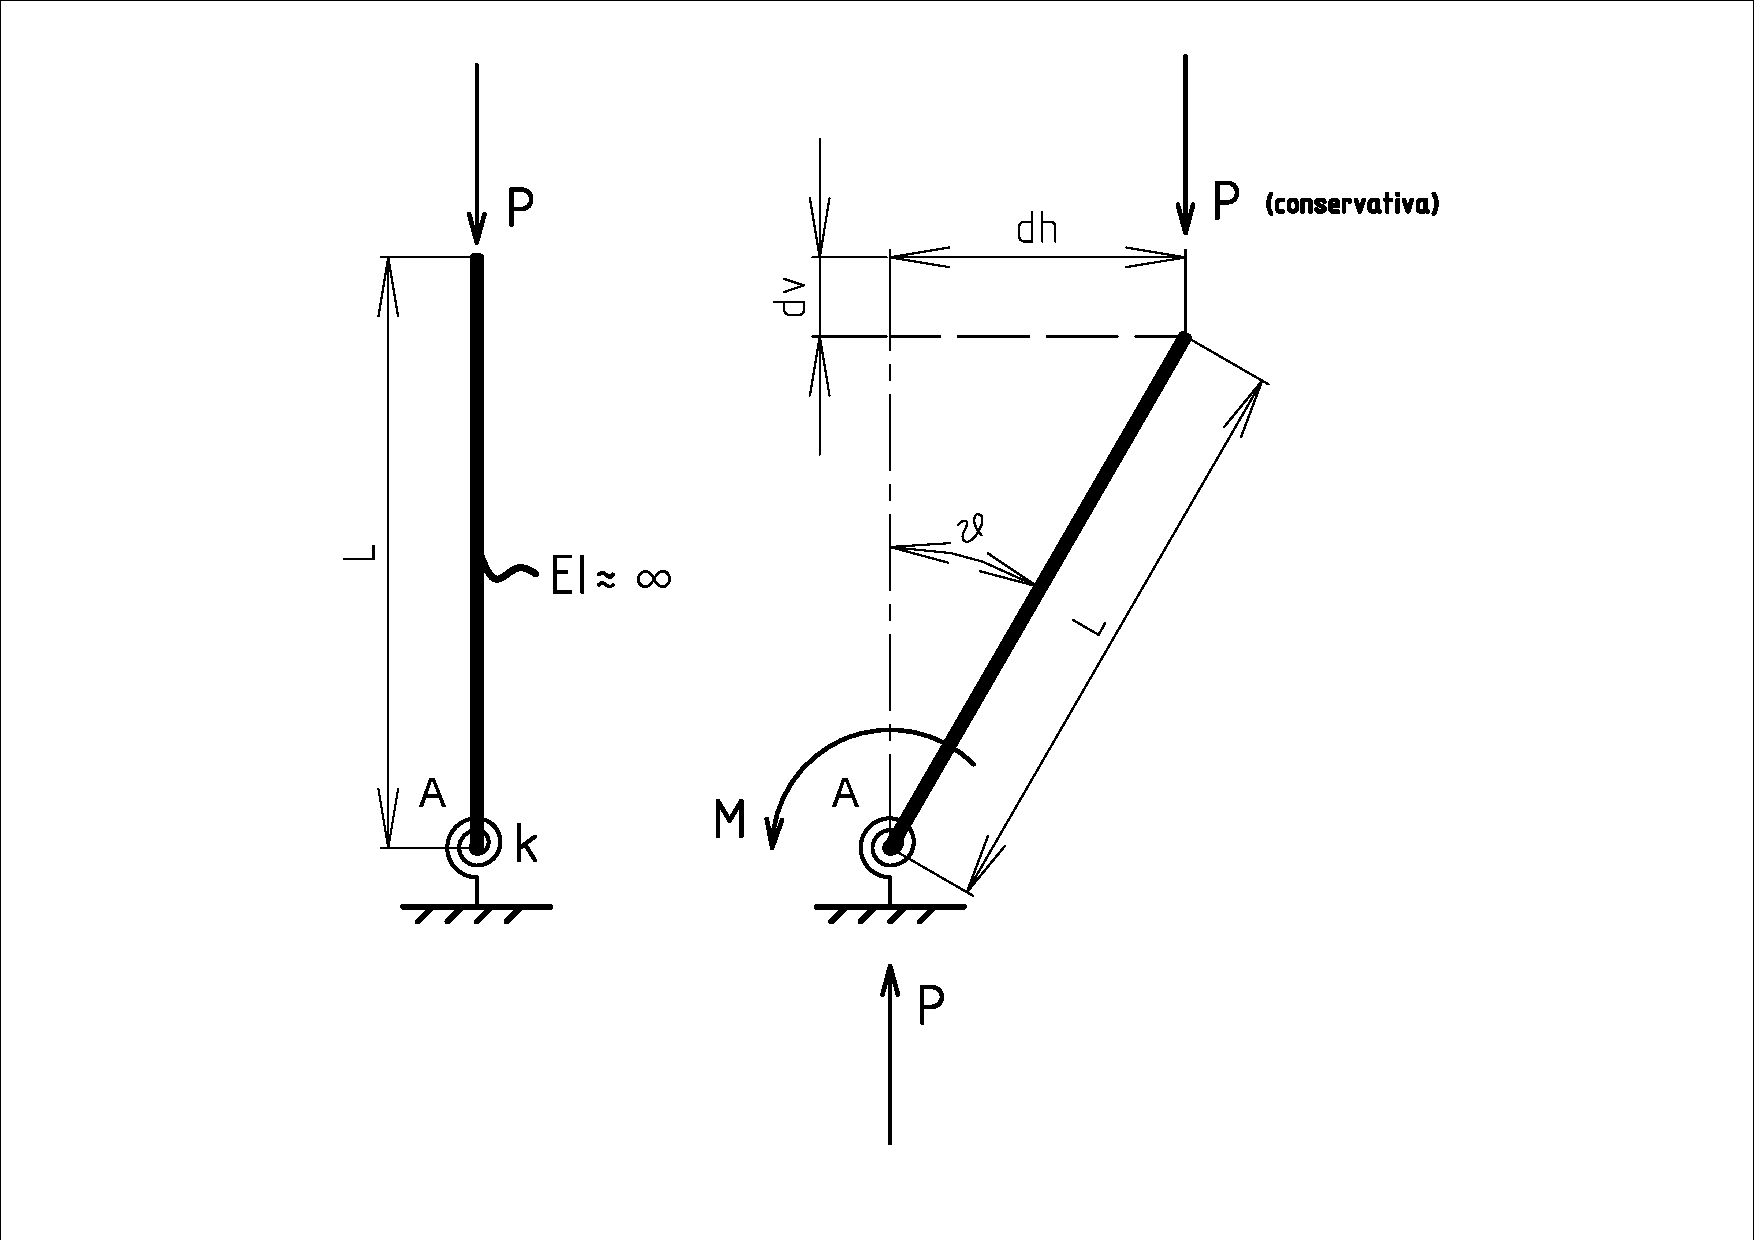
\includegraphics[
		trim=55mm 15mm 50mm 8mm,
		clip,
		width=0.73\textwidth
	]{figuras/TPs-1.pdf}
	\label{fig:TP1}
\end{figure}


% ================ Resolução TP-01 ================
\begin{textocaixa}
\hspace{10mm}
O sistema estrutural da barra rígida acoplada à uma mola de torção, de rigidez $K_\text{mola}$
na base, quando assumido possuir grandes deslocamentos, possui como solução geral para o
problema de determinação da carga $P$, aplicada verticalmente de forma conservativa na
extremidade livre da barra, a qual equilibra o sistema a expressão dada na
\autoref{eq:TP1-P_theta}.

\begin{equation}
	P = \frac{k_\text{mola}}{L}\frac{\theta}{\sin \theta}
	\label{eq:TP1-P_theta}
\end{equation}

Ainda, aplicando relações trigonométricas na geometria do sistema estrutural na condição de
equilíbrio, pode-se expressar o valor da carga em função dos deslocamentos vertical
($\delta_v$) e horizontal ($\delta_h$):

\begin{equation}
	\left\{\begin{array}{lcl}
		\delta_v &=& L\left(1 - \cos \theta\right) \\
		\delta_h &=& L\sin \theta \\
	\end{array}\right.
	\label{eq:TP1-deltavh}
\end{equation}

As fórmulas foram implementadas no MATLAB$^\text{\textregistered}$ para visualização gráfica
do comportamento não-linear geométrico (NLG) da estrutura, de acordo com os valores dados no
enunciado. Os gráficos $P\times\theta$, $P\times \delta_v$ e $P\times \delta_h$ são mostrados
na \autoref{fig:TP1-result}.

\begin{figure}[H]
	\centering
	\caption{TP1 $-$ Curvas do carregamento vertical $P$.}
	
\includegraphics[
		width=\textwidth
	]{figuras/no_image.png}
	\caption*{Fonte: Autor}
	\label{fig:TP1-result}
\end{figure}

As linhas de código que geraram estes gráficos estão disponíveis no \autoref{apendice:A}.

\end{textocaixa}